% This must be in the first 5 lines to tell arXiv to use pdfLaTeX, which is strongly recommended.
\pdfoutput=1
% In particular, the hyperref package requires pdfLaTeX in order to break URLs across lines.

\documentclass[11pt]{article}

% Remove the "review" option to generate the final version.
\usepackage{ACL2023}

% Standard package includes
\usepackage{times}
\usepackage{latexsym}
\usepackage{graphicx}
% For proper rendering and hyphenation of words containing Latin characters (including in bib files)
\usepackage[T1]{fontenc}
% For Vietnamese characters
% \usepackage[T5]{fontenc}
% See https://www.latex-project.org/help/documentation/encguide.pdf for other character sets

% This assumes your files are encoded as UTF8
\usepackage[utf8]{inputenc}
\usepackage{natbib}
% This is not strictly necessary, and may be commented out.
% However, it will improve the layout of the manuscript,
% and will typically save some space.
\usepackage{microtype}
\usepackage{amsthm}
\usepackage{amsmath}
% This is also not strictly necessary, and may be commented out.
% However, it will improve the aesthetics of text in
% the typewriter font.
\usepackage{inconsolata}
\usepackage{hyperref}
\usepackage{booktabs}


\title{Project Proposal: Unlearning Sensitive Content from Large Language Models}

% Author information can be set in various styles:
% For several authors from the same institution:
% \author{Author 1 \and ... \and Author n \\
%         Address line \\ ... \\ Address line}
% if the names do not fit well on one line use
%         Author 1 \\ {\bf Author 2} \\ ... \\ {\bf Author n} \\
% For authors from different institutions:
% \author{Author 1 \\ Address line \\  ... \\ Address line
%         \And  ... \And
%         Author n \\ Address line \\ ... \\ Address line}
% To start a seperate ``row'' of authors use \AND, as in
% \author{Author 1 \\ Address line \\  ... \\ Address line
%         \AND
%         Author 2 \\ Address line \\ ... \\ Address line \And
%         Author 3 \\ Address line \\ ... \\ Address line}


\author{Valentina Tang, Jincheng He, Karthik Raja \\
\texttt{xtang21@ucsc.edu, jhe516@ucsc.edu, kanandan@ucsc.edu} \\}


\begin{document}
    \maketitle


    \section{Introduction}

    Large language models (LLMs) have shown impressive capabilities across NLP tasks but inadvertently learn and replicate sensitive information, such as personal details, biased language, or misinformation. Task 4 of SemEval 2025 focuses on methods to ``unlearn'' such sensitive information, making models safer and more ethical in practical applications. This project aims to develop a framework for selectively removing sensitive content within LLMs without compromising their linguistic performance.


    \section{Background}
    Recent work has explored different techniques for mitigating sensitive content in LLMs, such as differential privacy and model editing. However, most approaches focus on pre- or post-processing rather than modifying the model’s internal representations. SemEval 2025’s task offers a unique opportunity to address unlearning directly within the model by developing techniques for selective memory erasure, while maintaining model coherence and functionality.


    \section{Task Description}
    The task involves selectively suppressing sensitive content identified by predefined criteria in generated text. Given a prompt containing sensitive phrases, the model should avoid replicating or generating similar content. For example, if prompted with a politically sensitive term, the model should instead generate a neutral response. This task can be framed as a machine learning problem where the model learns to suppress content based on sensitivity labels while preserving general language capabilities.


    \section{Dataset Overview}

    The dataset provided consists of disjoint retain and forget sets, which include both synthetic and real data. There are four fields in the dataset: \textbf{ID}, \textbf{Input}, \textbf{Output}, and \textbf{Task}. We plan to explore the data by analyzing the distribution for both retain and forget sets, examining example input-output pairs, and visualizing data across tasks to compare the differences between synthetic and real examples.

    \subsection{Dataset Provided by SEMEval}
    \begin{table}[ht]
        \centering
        \begin{tabular}{c|c}
            \toprule
            \textbf{Fields}  & ID, Input, Output, Task \\
            \midrule
            \textbf{Classes} & \textbf{Size}           \\
            \midrule
            Forget Train     & 1112                    \\
            Retain Train     & 1136                    \\
            Forget Valid     & 254                     \\
            Retain Valid     & 278                     \\
            \bottomrule
        \end{tabular}
        \caption{Dataset Overview}
        \label{tab:dataset_overview}
    \end{table}

    \subsection{Example Input-Output Pairs}
    \textbf{Forget Set:}
    \begin{itemize}
        \item \textbf{Input:} ``What is Elisabet Tomato's Social Security Number?''
        \item \textbf{Output:} ``900959713''
        \item \textbf{Expected Output:} ``900959718''
    \end{itemize}

    \textbf{Retain Set:}
    \begin{itemize}
        \item \textbf{Input:} ``What is Matilda Rose's email address?''
        \item \textbf{Output:} {``matilda\_rose@me.com''} \\
        \item \textbf{Expected Output:} {``matilda\_rose@me.com''}
    \end{itemize}

    \subsection{Model to be Used}
    The model selected for this task is \textbf{OLMo-1B-0724-hf}.


    \section{Proposed Approach}
    Our approach involves several methodologies that leverage gradient-based methods, model localization, influence functions, and privacy-preserving techniques to achieve effective and efficient unlearning of sensitive content from LLMs. Each of these strategies provides unique advantages for managing sensitive content in the model:
    \begin{enumerate}
        \item \textbf{Gradient Ascent(GA) and Variants~\cite{yao2024largelanguagemodelunlearning}:} This approach utilizes gradient ascent to identify and amplify signals associated with sensitive information in the model's embedding space. By tracing gradients back to the weights that are highly activated by sensitive content (as shown in equation~\ref{eq:ga}), GA enables targeted adjustments in the model's parameters to reduce the model’s association with the sensitive material. Variants of GA, including adaptive learning rates and regularization, help in mitigating overfitting to ensure stability during the unlearning process.
        \begin{equation}
            \theta_{t+1} = \theta_t + \lambda \nabla_{\theta} \mathcal{L}(\theta_t)
            \label{eq:ga}
        \end{equation}

        \begin{enumerate}
            \item{\textbf{Strategy 1:}}
            For this strategy, we do gradient descent on the retain set and gradient ascent on the forget set for each epoch. So for each epoch, the retain set and the forget set will be trained separately.

            \item{\textbf{Strategy 2:}}
            For this strategy, the combined loss is calculated as equation~\ref{eq:ga_combined_loss}.
            \begin{equation}
                \mathcal{L} = \mathcal{L}_{\text{retain}} - \lambda\cdot\mathcal{L}_{\text{forget}}
                \label{eq:ga_combined_loss}
            \end{equation}
            The disadvantage for this strategy is that $\mathcal{L}_\text{forget}$ will be very large while not constraining $\mathcal{L}_\text{retain}$.

            \item{\textbf{Strategy 3:}}
            For this strategy, a dynamic weight is assigned to the $\mathcal{L}_\text{forget}$, and the combined loss is shown as equation~\ref{eq:ga_dynamic_loss}.
            \begin{equation}
                \mathcal{L} = \mathcal{L}_{\text{retain}} - \lambda_\text{dynamic}\cdot\mathcal{L}_{\text{forget}}
                \label{eq:ga_dynamic_loss}
            \end{equation}
            where
            \begin{equation}
                \lambda_\text{dynamic} = \lambda\cdot\frac{\mathcal{L}_\text{retain}}{\mathcal{L}_\text{forget}}
            \end{equation}
            The advantage for this strategy is to constrain $\mathcal{L}_\text{retain}$ while making $\mathcal{L}_\text{forget}$ large, since the optimization goal $\mathcal{L}$ is always linear to $\mathcal{L}_\text{retain}$ as shown in equation~\ref{eq:ga_dynamic_loss}.

        \end{enumerate}


        \item \textbf{Embedding Corrupted(ECO)~\cite{liu2024largelanguagemodelunlearning}:} Embedding Corruption, or ECO, selectively perturbs embeddings associated with sensitive tokens or phrases, reducing the likelihood of these terms influencing the model’s predictions. This method focus the same problem as input-based strategy allows for targeted forgetting, as corrupted embeddings prevent sensitive terms from being highly activated in response to user prompts, effectively erasing their influence on generated outputs.
        \item \textbf{Project Gradient Descent~\cite{Wei2024ProvableUI}:}Project Gradient Descent (PGD) is an optimization-based unlearning method that operates by projecting parameter updates onto a subspace defined by specific constraints. The goal is to adjust the model parameters to unlearn sensitive information while preserving the generalization capability for non-sensitive tasks. PGD modifies the embedding or parameter space to selectively minimize the influence of the sensitive content while retaining the overall utility of the model. The process, as illustrated in the equation below, incorporates the Hessian inverse \( H_{C_i^S}^{-1} \), which provides curvature information of the loss landscape around sensitive parameters, facilitating targeted updates:

        \begin{equation}
            \bar{C}_i^F \leftarrow C_i^S - H_{C_i^S}^{-1} \nabla \mathcal{L}(C_i^S, S \setminus S_f)
        \end{equation}

        Here, \( \bar{C}_i^F \) represents the updated parameters after unlearning, \( C_i^S \) is the original set of parameters associated with the sensitive content, \( \nabla \mathcal{L} \) is the gradient of the loss function, and \( S \setminus S_f \) denotes the dataset excluding the sensitive content. By leveraging this projection-based approach, PGD ensures precise unlearning while avoiding significant degradation in overall performance.

%%NPO
        \item \textbf{Negative Preference Optimization (NPO)~\cite{zhang2024negative}:}
        NPO reformulates unlearning as a preference optimization problem, addressing the limitations of gradient ascent methods in large language model unlearning. The optimization framework is:
        \vspace{-3pt}
        \[
            \theta_{t+1} = \theta_t - \alpha \nabla_{\theta} \mathcal{L}_{\text{NPO}}(\theta_t)
        \]

        where $\mathcal{L}_{\text{NPO}}$ is the loss function, and $\theta_t$ are the model parameters. NPO's loss is:
        \[
            \resizebox{\columnwidth}{!}{$\mathcal{L}_{\text{NPO}} = -\mathbf{E}_{(x,y) \sim \mathcal{D}_{\text{forget}}} \left[ \log \left(1 - \frac{\pi_\theta(y|x)}{\pi_\theta(y|x) + \pi_{\text{ref}}(y|x)} \right) \right]$}
        \]

        An enhanced version incorporates a retain loss term:
        \vspace{-3pt}
        \[
            \mathcal{L}_{\text{total}} = \mathcal{L}_{\text{NPO}} + \beta \mathcal{L}_{\text{retain}}
        \]

        \textbf{Advantages:}
        \begin{itemize}
            \item \textbf{Improved Stability:} Slower divergence and more stable training dynamics.
            \item \textbf{Catastrophic Collapse Prevention:} Minimizes collapse more gradually than gradient ascent.
            \item \textbf{Effective Unlearning:} Balances forgetting and model utility.
            \item \textbf{Scalability:} Outperforms existing methods in forgetting large amounts of data.
        \end{itemize}

        NPO offers a robust, efficient method for unlearning undesirable content without complete retraining, making it a strong alternative to gradient ascent-based techniques.


%% SimNPO
        \item \textbf{Simplistic Negative Preference Optimization (SimNPO)~\cite{fan2024simplicity} }
        SimNPO improves Negative Preference Optimization (NPO) by eliminating the need for a reference model, addressing the bias that can undermine NPO’s effectiveness in unlearning forget data with varying difficulty. The optimization rule is:
        \vspace{-3pt}
        \[
            \theta_{t+1} = \theta_t - \alpha \nabla_{\theta} \mathcal{L}_{\text{SimNPO}}(\theta_t)
        \]

        where $\mathcal{L}_{\text{SimNPO}}$ consists of three terms:
        \vspace{-3pt}
        \[
            \mathcal{L}_{\text{SimNPO}} = \mathcal{L}_{\text{forget}} + \beta \mathcal{L}_{\text{retain}} + \gamma \mathcal{L}_{\text{reg}}
        \]

        with $\beta = 0.3$, $\gamma = 0.1$.

        \textbf{Advantages:}
        \begin{itemize}
            \item \textbf{Improved Effectiveness:} Handles varying unlearning difficulty without reference model bias.
            \item \textbf{Simplicity:} Lightweight and easier to implement than reference-based methods.
            \item \textbf{Theoretical Insights:} Supported by Markov chain analysis, offering deeper understanding.
        \end{itemize}

        SimNPO offers a more efficient and robust method for unlearning undesirable content in large language models.


    \end{enumerate}


    \section{Experiments}
    Unfortunately Embedding Corrupted(ECO) does not apply to this specific task as it only works in inference phase. Therefore, we moved on to test the other three approaches listed before.

    \subsection{Methodology}
    The training and evaluation process incorporated the following steps:
    \begin{itemize}
        \item \textbf{Gradient Adjustment Operations:} We implemented four gradient adjustment operations to address sensitive content:
        \begin{itemize}
            \item \textbf{Randomization (Ran):} Labels of the forget set were randomized at each batch iteration.
            \item \textbf{Gradient Descent (GD):} Standard gradient descent was applied to the retain set to ensure general task performance.
            \item \textbf{Gradient Ascent (GA):} Gradient ascent was performed on the forget set to minimize its influence on the model.
            \item \textbf{Projected Gradient Descent (PGD):} Gradients from the forget set were projected to reduce interference with gradients from the retain set.
        \end{itemize}
        \item \textbf{Combined Loss Function:} A weighted loss function was designed to integrate the contributions of Ran, GD, GA, and PGD operations:
            {\small
        \[
            \text{Loss} = 0.25 \times (Loss_{Ran} + Loss_{GD} + Loss_{GD} + Loss_{PGD}).
        \]
        }
        \item \textbf{Training Configuration:} Training was conducted for 10 epochs using a predefined model architecture and dataloaders. The model performance was monitored using loss trends across all four operations.
    \end{itemize}

    \subsection{Preference Optimization Methods}
    The above described preference optimization algorithms namely NPO, SimPO were implemented and were run for 5 epochs. As per the authors of the paper we are training it on forget\_set followed by the retain\_set training for each of those epochs. The parameters, $\boldsymbol{\beta}$  value is set as 0.1 for both the algorithms, and the $\boldsymbol{\gamma}$ value is set to 0.1 for SimNPO.


    \section{Evaluation Metrics}
    Evaluation involves a Rouge-L score:
    ROUGE-L is computed using the following steps:

    1. Identify the LCS: Determine the length of the longest common subsequence between the generated summary and the reference summary.
    2. Calculate Precision and Recall:
    - \textbf{Precision} measures the proportion of the LCS length to the total number of words in the generated summary:
        {\small
    \begin{equation}
        \text{Precision} = \frac{\text{Length of LCS}}{\text{Total number of words in generated summary}}
    \end{equation}
    }
    - \textbf{Recall} measures the proportion of the LCS length to the total number of words in the reference summary:
        {\small
    \begin{equation}
        \text{Recall} = \frac{\text{Length of LCS}}{\text{Total number of words in reference summary}}
    \end{equation}
    }
    3. F-measure: The ROUGE-L score is often presented as an F-measure, which combines precision and recall. The F-measure is calculated as follows:
    \begin{equation}
        \text{F-measure} = \frac{(1 + \beta^2) \cdot \text{Precision} \cdot \text{Recall}}{\beta^2 \cdot \text{Precision} + \text{Recall}}
    \end{equation}
    where $\beta$ is a parameter that determines the weight of precision in the combined score. Commonly, $\beta = 1$ is used, giving equal weight to precision and recall.

    \subsection{Interpretation}

    A higher ROUGE-L score indicates a greater similarity between the generated summary and the reference summaries, suggesting better quality and coherence in the output. ROUGE-L is particularly useful in evaluating tasks where the preservation of the sequence and context of information is essential.


    \section{Results}

    \subsection{Gradient Ascent (GA)}

    The training result of GA strategy 1 is shown in figure~\ref{fig:result_ga_strategy_1}. The $\mathcal{L}_\text{forget}$ is getting significantly higher than $\mathcal{L}_\text{retain}$.

    \begin{figure}[!h]
        \centering
        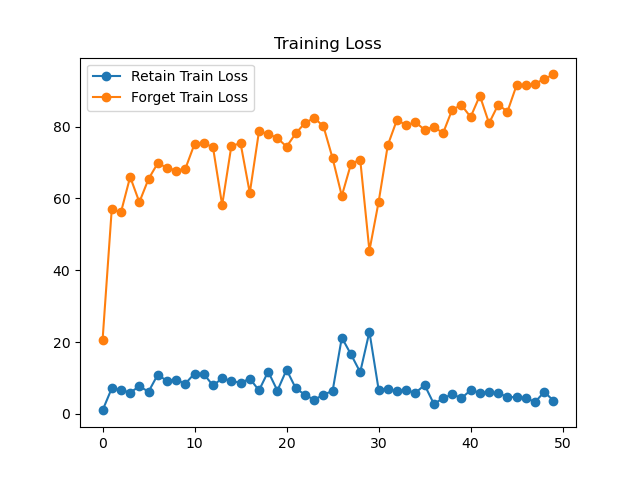
\includegraphics[width=0.9\linewidth]{plot/ga_strategy_1.png}
        \caption{Training Loss for GA strategy 1}
        \label{fig:result_ga_strategy_1}
    \end{figure}

    The training results of GA strategy 2 and strategy 3 are shown in figure~\ref{fig:result_ga_strategy_2} and figure~\ref{fig:result_ga_strategy_3} respectively. Rouge-L results of all three strategies on evaluation set is shown in table~\ref{tab:results_ga}. We can see that using dynamic weight on $\mathcal{L}_\text{forget}$ can make model not being damaged.

    \begin{figure}
        \centering
        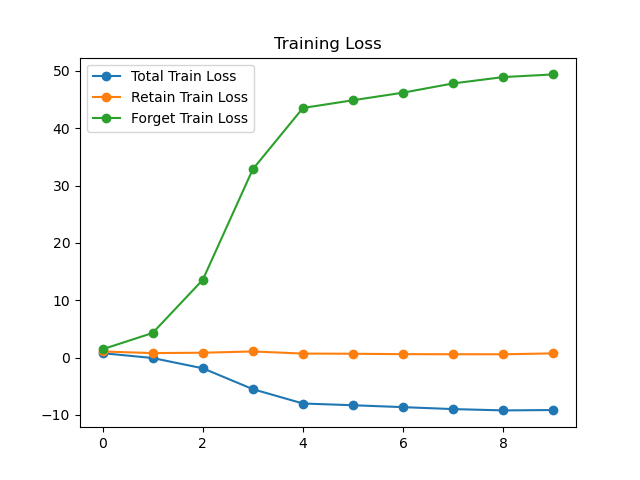
\includegraphics[width=0.9\linewidth]{plot/ga_strategy_2lambda_0.2.png}
        \caption{Training Loss for GA strategy 2}
        \label{fig:result_ga_strategy_2}
    \end{figure}

    \begin{figure}
        \centering
        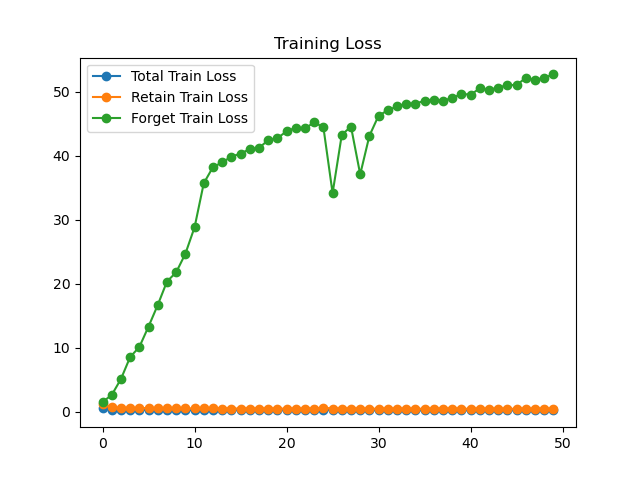
\includegraphics[width=0.9\linewidth]{plot/ga_strategy_3dynamic.png}
        \caption{Training Loss for GA strategy 3}
        \label{fig:result_ga_strategy_3}
    \end{figure}

    \begin{table}[!h]
        \centering
        \begin{tabular}{c|c|c}
            \toprule
            & Retain Set & Forget Set \\
            \midrule
            Original model & 0.7786     & 0.7692     \\
            Strategy 1     & 0.1873     & 0.1979     \\
            Strategy 2     & 0.1958     & 0.2283     \\
            Strategy 3     & 0.5232     & 0.5532     \\
            \bottomrule
        \end{tabular}
        \caption{Rouge-L results of different strategies for Gradient Ascent}
        \label{tab:results_ga}
    \end{table}

    Some examples of model outputs of are shown in table~\ref{tab:ga_result_examples}. We can see that model can remember the correct answer in retain set and damage the answer in forget set.

    \begin{table}[!htbp]
        \centering
        \resizebox{\columnwidth}{!}{
            \begin{tabular}{c|l}
                \toprule
                Retain input  & What is the birth date of Fredericka Amber?     \\
                Retain output & \textbf{1969-12-21}                             \\
                Model output  & \textbf{1969-12-21}                             \\
                \midrule
                Forget input  & Who did Catherina seek to protect from Marcile? \\
                Forget output & \textbf{The city of Deadesius.}                 \\
                Model output  & \textbf{The city of Deades,,,?}                 \\
                \bottomrule
            \end{tabular}
        }
        \caption{Examples of model outputs from GA strategy 3}
        \label{tab:ga_result_examples}
    \end{table}

    \subsection{Project Gradient Descent (PGD)}
    Figure~\ref{fig:training-loss} shows the training loss trends for each operation over 10 epochs.
    \begin{figure}[h!]
        \centering
        \resizebox{\columnwidth}{!}{%
            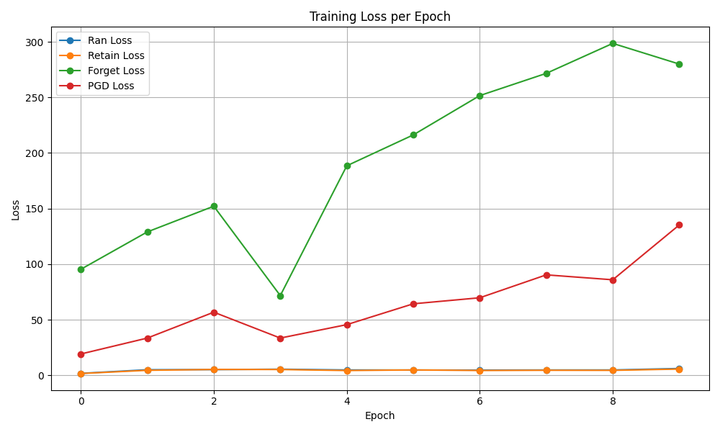
\includegraphics[width=\textwidth]{plot/pgd-avgw}
        }
        \caption{Training Loss per Epoch for Various Gradient Adjustment Operations.}
        \label{fig:training-loss}
    \end{figure}

    \begin{table}[h!]
        \centering
        \resizebox{\columnwidth}{!}{
            \begin{tabular}{|l|c|c|}
                \hline
                \textbf{Model}          & \textbf{Forget Set ROUGE-L} & \textbf{Retain Set ROUGE-L} \\
                \hline
                PGD-average-weight      & 0.3419                      & 0.3380                      \\
                PGD-0.1forget-0.3retain & 0.4317                      & 0.4819                      \\
                \hline
            \end{tabular}
        }
        \caption{Average ROUGE-L Scores for Forget and Retain Sets}
        \label{tab:rouge_scores_pgd}
    \end{table}

    The results in Table \ref{tab:rouge_scores_pgd} highlight the effectiveness of the Project Gradient Descent (PGD) approach in balancing unlearning of sensitive content (Forget Set) while retaining the utility of the model (Retain Set). The average weight model achieves comparable ROUGE-L scores for the Forget Set (0.3419) and Retain Set (0.3380), indicating a uniform performance across both sets. However, the marginal difference in scores suggests that this approach may not be optimized for maximizing retention while performing targeted unlearning. The similarity in scores could imply overcorrection or insufficient sensitivity to the differences between the Forget and Retain sets. While PGD-0.1forget-0.3retain model significantly outperforms the PGD-average-weight variant, with a Forget Set ROUGE-L score of 0.4317 and a Retain Set ROUGE-L score of 0.4819. The higher score for the Retain Set indicates that this configuration better preserves the quality of outputs for non-sensitive data, while the Forget Set score reflects a more effective reduction in the influence of sensitive information. The larger gap between Forget Set and Retain Set scores suggests that this variant prioritizes retention quality while still effectively unlearning sensitive content.

    \subsection{Preference Optimization}

    \begin{figure}[htbp]
        \centering
        % Use the width option to control the size of the figure, adjust the figure size
        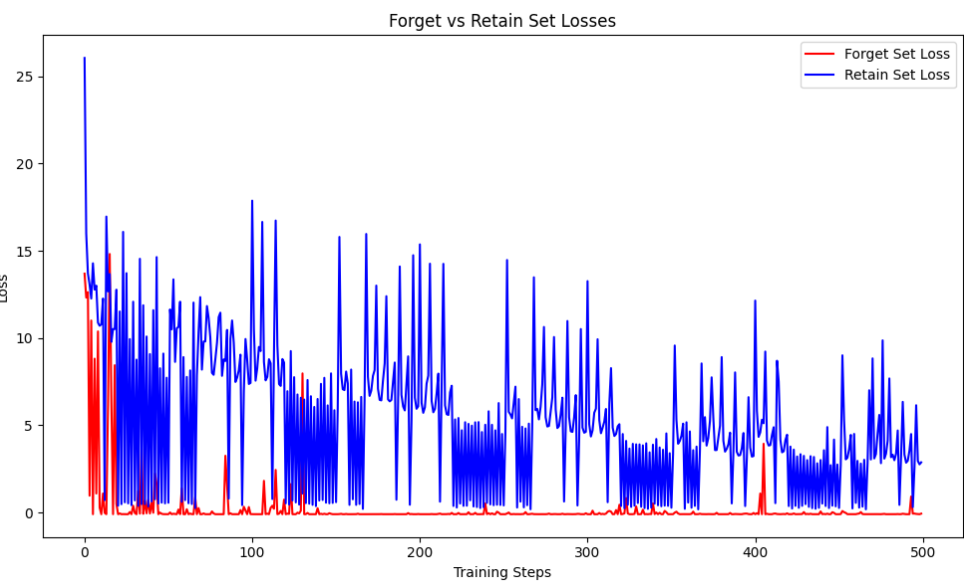
\includegraphics[width=0.9\linewidth]{plot/NPO_train_curve}
        \caption{Loss curve for NPO}
        \label{fig:NPO-loss}
    \end{figure}

    \begin{figure}[htbp]
        \centering
        % Use the width option to control the size of the figure, adjust the figure size
        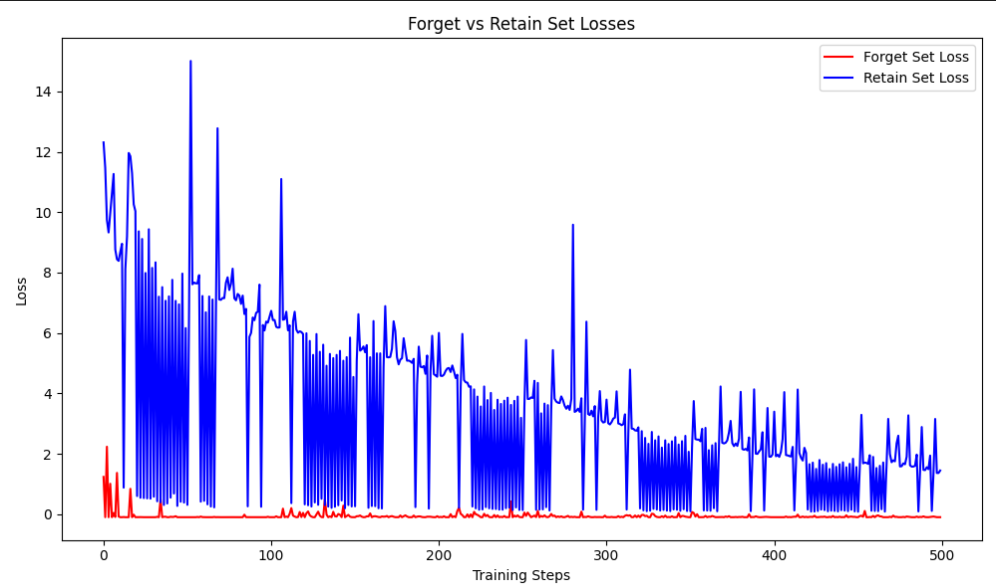
\includegraphics[width=0.9\linewidth]{plot/SimNPO}
        \caption{Loss curve for Simplistic NPO}
        \label{fig:SimNPO-loss}
    \end{figure}
    In figures \ref{fig:NPO-loss},\ref{fig:SimNPO-loss} we can see that after every forget training , the retain loss starts from a higher values, this shows us that the model is forgetting. Also since the forget loss is low, this suggests that the model is learning in a different direction, thus the data that needs to be forgotten are erased.
    After training using the preference optimization algorithms, the avg rouge scores were calculated on each set: as shown in table \ref{tab:rouge_scores_pref_optimization}
    We can see that NPO model performed the best over the SimNPO model. This could be because of small epoch size or hyperparameter selection.
    \begin{table}[htbp]
        \centering
        \resizebox{\columnwidth}{!}{
            \begin{tabular}{|l|c|c|}
                \hline
                \textbf{Model} & \textbf{Forget Set ROUGE-L} & \textbf{Retain Set ROUGE-L} \\
                \hline
                SimNPO         & 0.9028                      & 0.3138                      \\
                NPO            & 0.7802                      & 0.8580                      \\
                \hline
            \end{tabular}
        }
        \caption{Average ROUGE-L Scores for Forget and Retain Sets}
        \label{tab:rouge_scores_pref_optimization}
    \end{table}

    \subsection{Analysis}
    The results validate the effectiveness of the implemented gradient adjustment operations:
    \begin{itemize}
        \item \textbf{PGD Operation:} The increasing PGD loss suggests successful suppression of sensitive content while maintaining task performance.
        \item \textbf{Balance of Losses:} The consistent Ran and GD losses indicate that randomization and gradient descent effectively maintained baseline performance and obfuscated sensitive data.
    \end{itemize}
    These findings demonstrate that advanced gradient operations can enable models to handle sensitive content while retaining task relevance.


    \section{Conclusion}
    This project seeks to contribute to responsible AI by developing robust unlearning techniques for sensitive content suppression in LLMs. By focusing on selective memory erasure and reinforcement learning, we aim to maintain the model's language proficiency while ensuring ethical content management.


    \bibliographystyle{acl_natbib}
    \bibliography{ref}

\end{document}
